% Tikz File 'tikz_pic_14.tex'
\documentclass{standalone}
\usepackage{tikz}
\usetikzlibrary{arrows}
\usetikzlibrary{shapes.misc}
\usetikzlibrary{decorations.markings}
\tikzset{cross/.style={cross out, draw=black, minimum size=2*(#1-\pgflinewidth), inner sep=0pt, outer sep=0pt},cross/.default={1pt}}
\tikzset{
    halfarrow1/.style={postaction={decorate},
        decoration={markings,mark=at position .5 with
        {\arrow[line width=0.4mm]{>}}}} }
\tikzset{
    halfarrow2/.style={postaction={decorate},
        decoration={markings,mark=at position .5 with
        {\arrow[line width=0.4mm]{<}}}} }
\begin{document}
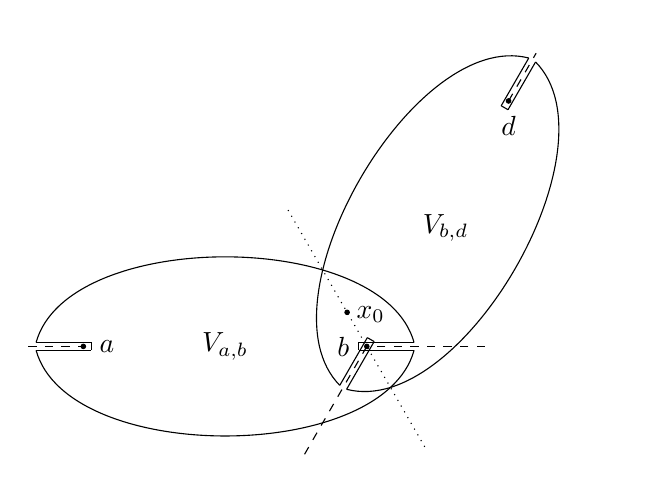
\begin{tikzpicture}

    

% \draw (-1.8,1.0) node {$\Phi(\tilde{\alpha})$};  \draw (2,-1.3) node {$\Phi(\tilde{\beta})$};
  \draw (-3.3,0) node {$a$};  \draw (-0.3,0) node {$b$}; \draw (-1.8,0) node {$V_{a,b}$};
  \filldraw [black] (-3.6,0) circle (0.8pt); \filldraw [black] (0,0) circle (0.8pt);
    \draw [dashed] (-4.3,0) -- (-3.6,0);   \draw [dashed] (1.5,0) -- (0,0);
    \draw (-4.2,0.05) .. controls (-3.8,1.5) and (0.2,1.5) .. (0.6,0.05);
    \draw (-4.2,-0.05) .. controls (-3.8,-1.5) and (0.2,-1.5) .. (0.6,-0.05);
    \draw (-4.2,-0.05) -- (-3.5,-0.05); \draw (0.6,-0.05) -- (-0.1,-0.05);
    \draw (-4.2,0.05) -- (-3.5,0.05); \draw (0.6,0.05) -- (-0.1,0.05);
    \draw (-3.5,0.05) -- (-3.5,-0.05); \draw (-0.1,0.05) -- (-0.1,-0.05);
    
  \filldraw [black] (1.8,3.117) circle (0.8pt); 
  \draw (1.8,2.8) node {$d$}; \draw (1.0,1.5) node {$V_{b,d}$};
  \draw [dashed] (1.8,3.117) -- (2.15,3.723); \draw [dashed] (0,0) -- (-0.8,-1.386);
  \draw [rotate=240,shift={(0,0)}] (-4.2,0.05) .. controls (-3.8,1.5) and (0.2,1.5) .. (0.6,0.05);
  \draw [rotate=240,shift={(0,0)}] (-4.2,-0.05) .. controls (-3.8,-1.5) and (0.2,-1.5) .. (0.6,-0.05);
  \draw [rotate=240,shift={(0,0)}] (-4.2,-0.05) -- (-3.5,-0.05);  \draw [rotate=240,shift={(0,0)}] (0.6,-0.05) -- (-0.1,-0.05);
    \draw [rotate=240,shift={(0,0)}](-4.2,0.05) -- (-3.5,0.05); \draw [rotate=240,shift={(0,0)}] (0.6,0.05) -- (-0.1,0.05);
       \draw [rotate=240,shift={(0,0)}] (-3.5,0.05) -- (-3.5,-0.05); \draw [rotate=240,shift={(0,0)}] (-0.1,0.05) -- (-0.1,-0.05);
       
  \draw [dotted] (-1,1.732) -- (0.75,-1.3);
  \filldraw [black] (-0.25,0.433) circle (0.8pt); \draw (0.05,0.4) node {$x_0$};
%   \draw (3.6*0.5+0.2,3.6*-0.866) node {$d$}; \draw [black] (0.0,-0.4) node {$x$}; 
%    \filldraw [black] (-3.6,0) circle (1pt); \filldraw [black] (0,0) circle (1pt); \filldraw [black] (3.6*0.5,3.6*-0.866) circle (1pt); \filldraw [black] (-0.22,-0.38) circle (1pt); 
%  \draw [black] (-3.6,0) -- (0,0); \draw [black] (0,0) -- (3.6*0.5,3.6*-0.866); \draw[dashed]
%  (0,0) -- (1.4,0); \draw [dotted] (0,0) -- (-2*0.5,2*-0.866);
%  \draw [dashed] (0,0) -- (-0.7,1.21);
%  \draw [black] (-0.025,-0.043) -- (0.625,-0.043);
% \draw [black] (-0.025,-0.043) -- (-0.315,0.455);
%  \draw [black] (0.625,-0.043) arc (0:-236:0.6cm);
 %\draw (-3.6,0) .. controls (-1.8,0.3) and (-1.8,0.3) .. (0.0,0.0) [halfarrow2];
%  \draw (-3.6,0) .. controls (-0.2,-0.6) and (-0.2,-0.6) .. (0.0,0.0) [halfarrow1];
% \draw [rotate=-60,shift={(3.6,0)}] (-3.6,0) .. controls (-1.8,0.3) and (-1.8,0.3) .. (0.0,0.0) [halfarrow2];
% \draw [rotate=-60,shift={(3.6,0)}] (-3.6,0) .. controls (-3.4,-0.6) and (-3.4,-0.6) .. (0.0,0.0) [halfarrow1];
%  \draw (1,0.0) arc (0:-60:1cm) [->]; \draw (1.1,-0.5) node {$\tau$};
%   \draw (-1,0.0) arc (180:240:1cm) [->]; \draw (-1.1,-0.8) node {$\frac{\pi+\tau}{2}$};

 
\end{tikzpicture}
\end{document}
